\documentclass[spanish,a4paper,11pt,twoside]{report}

%%%%%%%%%%%%%%%%%%%%%%%%%%%%%%%%%%%%%%%%%%%%%%%%%%%%%%%%%%%%%%%%%%%%%%%%%%%%%%%
\usepackage[dvips]{graphicx}
\usepackage[dvips]{epsfig}
\usepackage[utf8]{inputenc}
\usepackage[english]{babel}
\usepackage{alltt}
\usepackage{templates/algorithm}
\usepackage{templates/algorithmic}
\usepackage{templates/multirow}

%%%%%%%%%%%%%%%%%%%%%%%%%%%%%%%%%%%%%%%%%%%%%%%%%%%%%%%%%%%%%%%%%%%%%%%%%%%%%%%

\newcommand{\SONY}{{\sc Sony}}
\newcommand{\MICROSOFT}{{\sc Microsoft}}
\newcommand{\GCC}{\textsf{\textsc{G}CC}}
\newcommand{\INTEL}{\textsf{\textsc{I}ntel}}

%%% Traducimos el pseudocodigo
\renewcommand{\algorithmicwhile}{\textbf{mientras}}
\renewcommand{\algorithmicend}{\textbf{fin}}
\renewcommand{\algorithmicdo}{\textbf{hacer}}
\renewcommand{\algorithmicif}{\textbf{si}}
\renewcommand{\algorithmicthen}{\textbf{entonces}}
\renewcommand{\algorithmicrepeat}{\textbf{repetir}}
\renewcommand{\algorithmicuntil}{\textbf{hasta que}}
\renewcommand{\algorithmicelse}{\textbf{en otro caso}}
\renewcommand{\algorithmicfor}{\textbf{para}}

%\newcommand{\RETURN}{\textbf{retornar} }
\newcommand{\RET}{\STATE \textbf{retornar} }
\newcommand{\TO}{\textbf{hasta} }
\newcommand{\AND}{\textbf{y} }
\newcommand{\OR}{\textbf{o} }

%%%%%%%%%%%%%%%%% Creamos un entorno para listar código fuente %%%%%%%%%%%%%%%
\newenvironment{sourcecode}
{\begin{list}{}{\setlength{\leftmargin}{1em}}\item\scriptsize\bfseries}
{\end{list}}

\newenvironment{littlesourcecode}
{\begin{list}{}{\setlength{\leftmargin}{1em}}\item\tiny\bfseries}
{\end{list}}

\newenvironment{summary}
{\par\noindent\begin{center}\textbf{Abstract}\end{center}\begin{itshape}\par\noindent}
{\end{itshape}}

\newenvironment{keywords}
{\begin{list}{}{\setlength{\leftmargin}{1em}}\item[\hskip\labelsep \bfseries Keywords:]}
{\end{list}}

\newenvironment{palabrasClave}
{\begin{list}{}{\setlength{\leftmargin}{1em}}\item[\hskip\labelsep \bfseries Palabras clave:]}
{\end{list}}


%%%%%%%%%%%%%%%%%%%%%%%%%%%%%%%%%%%%%%%%%%%%%%%%%%%%%%%%%%%%%%%%%%%%%%%%%%%%%%%
% Format
%%%%%%%%%%%%%%%%%%%%%%%%%%%%%%%%%%%%%%%%%%%%%%%%%%%%%%%%%%%%%%%%%%%%%%%%%%%%%%%

%%\topmargin -4 mm
%\topmargin -21 mm
%\headheight 10 mm
%\headsep 10 mm

%\textheight 229 mm
%\textheight 246 mm

%\oddsidemargin -5.4 mm
%\evensidemargin -5.4 mm
\oddsidemargin 5 mm
\evensidemargin 5 mm

%\oddsidemargin -3 mm
%\evensidemargin -3 mm

%\textwidth 17 cm
\textwidth 15 cm
%\columnsep 10 mm

\input{amssym.def}

%%%%%%%%%%%%%%%%%%%%%%%%%%%%%%%%%%%%%%%%%%%%%%%%%%%%%%%%%%%%%%%%%%%%%%%%%%%%%%%

\begin{document}

%%%%%%%%%%%%%%%%%%%%%%%%%%%%%%%%%%%%%%%%%%%%%%%%%%%%%%%%%%%%%%%%%%%%%%%%%%%%%%%
% First Page 
%%%%%%%%%%%%%%%%%%%%%%%%%%%%%%%%%%%%%%%%%%%%%%%%%%%%%%%%%%%%%%%%%%%%%%%%%%%%%%%

\pagestyle{empty}
\thispagestyle{empty}


\newcommand{\HRule}{\rule{\linewidth}{1mm}}
\setlength{\parindent}{0mm}
\setlength{\parskip}{0mm}
\vspace*{\stretch{1}}

\begin{center}
\includegraphics[width=0.2\textwidth]{images/logotipo-secundario-ULL}\\[0.25cm]
\end{center}

\HRule
\begin{center}
        {\Huge Proyecto de la asignatura Computacion Avanzada } \\[2.5mm] 
        {\Huge Título del Artículo :  A parallel tabu search algorithm for solving
the container loading problem
} \\[5mm]

        {\Large Autor : ROBABEH SALEHI} \\[10mm]

        {\em Computación Avanzada} \\[5mm]
        Lenguajes y Sistemas Informáticos \\[5mm]
        Escuela Técnica Superior de Ingeniería y Tecnología \\[5mm]
        
        Universidad de La Laguna \\
\end{center}
\HRule
\vspace*{\stretch{2}}
\begin{center}
  La Laguna, \today 
\end{center}

%%%%%%%%%%%%%%%%%%%%%%%%%%%%%%%%%%%%%%%%%%%%%%%%%%%%%%%%%%%%%%%%%%%%%%%%%%%%%%%
\begin{abstract}
{\em

%El objetivo de este trabajo ha sido ....
%
%bla, bla, bla
%
%bla, bla, bla
%
%bla, bla, bla
Abstract
This paper presents a parallel tabu search algorithm for the container loading problem with
a single container to be loaded. The emphasis is on the case of a weakly heterogeneous load.
The distributed-parallel approach is based on the concept of multi-search threads according to
Toulouse et al. [Issues in designing parallel and distributed search algorithms for discrete optimization
problems, Publication CRT-96-36, Centre de recherche sur les transports, Universitede
Montreal, Canada, 1996] i.e., several search paths are investigated concurrently. The
parallel searches are carried out by differently configured instances of a tabu search algorithm,
which cooperate by the exchange of (best) solutions at the end of defined search phases. The
parallel search processes are executed on a corresponding number of LAN workstations. The
efficiency of the parallel tabu search algorithm is demonstrated by an extensive comparative
test including well-known reference problems and loading procedures from other authors.
 2003 Elsevier Science B.V. All rights reserved.



In the interest of stability of the load, both horizontal dimensions of each box are
to be supported according to a predefined percentage. In any case the centre of gravity
of each box must be supported in order to avoid boxes tipping over. It is assumed
that the centre of gravity and the geometric centre of each box coincide.
Box types are defined as follows. Two boxes are the same type if they coincide in
all three side dimensions. On the basis of this concept of box types, the following
three categories of box sets can be distinguished. A homogeneous box set is given
if all boxes are of the same type. A box set is called weakly heterogeneous if there
exist a few box types and many items per type. Finally, a strongly heterogeneous
box set is characterized by a greater number of box types and only few items per
type. Here, a weakly heterogeneous set of boxes is assumed.
In the recent years, many (sequential) solution methods for the container loading
problem have been developed. It is well known that the container loading problem is
NP-hard (cf. [18]). Hence, the methods developed are heuristic approaches.

The only block of a 1-arrangement is always placed in the reference corner of the
packing space. From the two blocks of a 2-arrangement, one is arranged in the
reference corner. The second block can alternatively be placed as a neighbour in
x-direction (arrangement type ‘‘in front of’’), as a neighbour in y-direction (arrangement
type ‘‘beside’’) or as a neighbour in z-direction (arrangement type ‘‘above’’). In
the case of a placement according to arrangement type ‘‘in front of’’, the block with
the larger y-dimension is positioned in the reference corner, while for the arrangement
type ‘‘beside’’ the block with the larger x-dimension is positioned in the reference
corner. The arrangement type ‘‘above’’ is only used if both horizontal
dimensions of a block are not smaller than the corresponding dimensions of the
other block. The block with the larger horizontal dimensions is positioned in the reference
corner and the other above. Fig. 2 illustrates a 1-arrangement and two 2-
arrangements of the arrangement types ‘‘in front of’’ and ‘‘beside’’.

}

\begin{palabrasClave}
Tabu searchin: is one of the searching method.
\end{palabrasClave}

\end{abstract}
%%%%%%%%%%%%%%%%%%%%%%%%%%%%%%%%%%%%%%%%%%%%%%%%%%%%%%%%%%%%%%%%%%%%%%%%%%%%%%%

%%%%%%%%%%%%%%%%%%%%%%%%%%%%%%%%%%%%%%%%%%%%%%%%%%%%%%%%%%%%%%%%%%%%%%%%%%%%%%%
%\newpage{\pagestyle{empty}\cleardoublepage}

\pagestyle{myheadings} %my head defined by markboth or markright
% No funciona bien \markboth sin "twoside" en \documentclass, pero al
% ponerlo se dan un mont�n de errores de underfull \vbox, con lo que no se
% ha puesto.
\markboth{ROBABEH SALEHI}{A parallel tabu search algorithm for solving
the container loading problem}

%%%%%%%%%%%%%%%%%%%%%%%%%%%%%%%%%%%%%%%%%%%%%%%%%%%%%%%%%%%%%%%%%%%%%%%%%%%%%%%
%Numeracion en romanos
\renewcommand{\thepage}{\roman{page}}
\setcounter{page}{1}


%\tableofcontents

%%%%%%%%%%%%%%%%%%%%%%%%%%%%%%%%%%%%%%%%%%%%%%%%%%%%%%%%%%%%%%%%%%%%%%%%%%%%%%%

%\listoffigures

%%%%%%%%%%%%%%%%%%%%%%%%%%%%%%%%%%%%%%%%%%%%%%%%%%%%%%%%%%%%%%%%%%%%%%%%%%%%%%%

%\listoftables

%%%%%%%%%%%%%%%%%%%%%%%%%%%%%%%%%%%%%%%%%%%%%%%%%%%%%%%%%%%%%%%%%%%%%%%%%%%%%%%
%\newpage{\pagestyle{empty}\cleardoublepage}

%%%%%%%%%%%%%%%%%%%%%%%%%%%%%%%%%%%%%%%%%%%%%%%%%%%%%%%%%%%%%%%%%%%%%%%%%%%%%%%
%Numeracion a partir del capitulo I
\renewcommand{\thepage}{\arabic{page}}
\setcounter{page}{1}

\setlength{\parindent}{5mm}

%%%%%%%%%%%%%%%%%%%%%%%%%%%%%%%%%%%%%%%%%%%%%%%%%%%%%%%%%%%%%%%%%%%%%%%%%%%%%%%
\chapter{Heuristic Algorithm}
\label{chapter:obj}

%%%%%%%%%%%%%%%%%%%%%%%%%%%%%%%%%%%%%%%%%%%%%%%%%%%%%%%%%%%%%%%%%%%%%%%%%%%%%
% Chapter 1:  
%%%%%%%%%%%%%%%%%%%%%%%%%%%%%%%%%%%%%%%%%%%%%%%%%%%%%%%%%%%%%%%%%%%%%%%%%%%%%%%

By means of the basic heuristic a given container is loaded in several iterations.
Within an iteration a so-called packing space is filled with one or more boxes.
A packing space is an empty rectangular space within the container with defined side
dimensions. In the first iteration the complete interior of the container is used as the
packing space. For the loading of a packing space only box arrangements with a predefined
simple structure are considered. These are called local arrangements. The
feasible local arrangements for a packing space are generated and evaluated by
means of certain criteria. The unused part of the packing space is completely subdivided
into several residual packing spaces. These are filled later. A rough description
of the algorithm of the basic heuristic is given in Fig. 1.
The overall algorithm presented in Fig. 1 requires some comments.

• In order to enhance the chances of loading small packing spaces, the packing
space with the smallest volume is always processed first.

• The container is embedded in a three-dimensional coordinates system. The bottom
left-hand rear corner of a packing space is used as the reference corner.
The coordinates of the reference corner are stored together with the dimensions
of the packing space. The position of a box results from the coordinates of the
reference corner of the respective packing space and its placement within the respective
local arrangement (see below).

• In this section, the basic heuristic is presented as a greedy heuristic. In step (5) the
best evaluated first local arrangement of ArrList is selected. In Section 3 the basic
heuristic is extended in such a way that the best arrangement is not necessarily
used for a packing space with packing space index ipr. Only with this extension
can the basic heuristic be used for the generation of different solutions to a prob-
lem instance. It should be mentioned that an index ipr is only assigned to fillable
packing spaces in which at least one box can be placed.

• At the same time as a local arrangement is generated and evaluated (step 2), the
residual packing spaces that would occur if this local arrangement was used are
generated. In step (6) these residual packing spaces are possibly inserted into
the packing space list PrList.
From the last comment it can be concluded that a more detailed description of the
basic heuristic requires merely a refinement of step (3), which is subsequently described.


%---------------------------------------------------------------------------------
%\section{Sección Uno}
%\label{1:sec:1}
%  Primer párrafo de la primera sección.


%---------------------------------------------------------------------------------
%\section{Sección Dos}
%\label{1:sec:2}
%  Primer párrafo de la segunda sección.

%\begin{itemize}
%  \item Item 1
%  \item Item 2
%  \item Item 3
%\end{itemize}


%""""""""""""""""""""""""""""""""""""""""""""""""""""""""""""""""""""""""""""""
\begin{center}
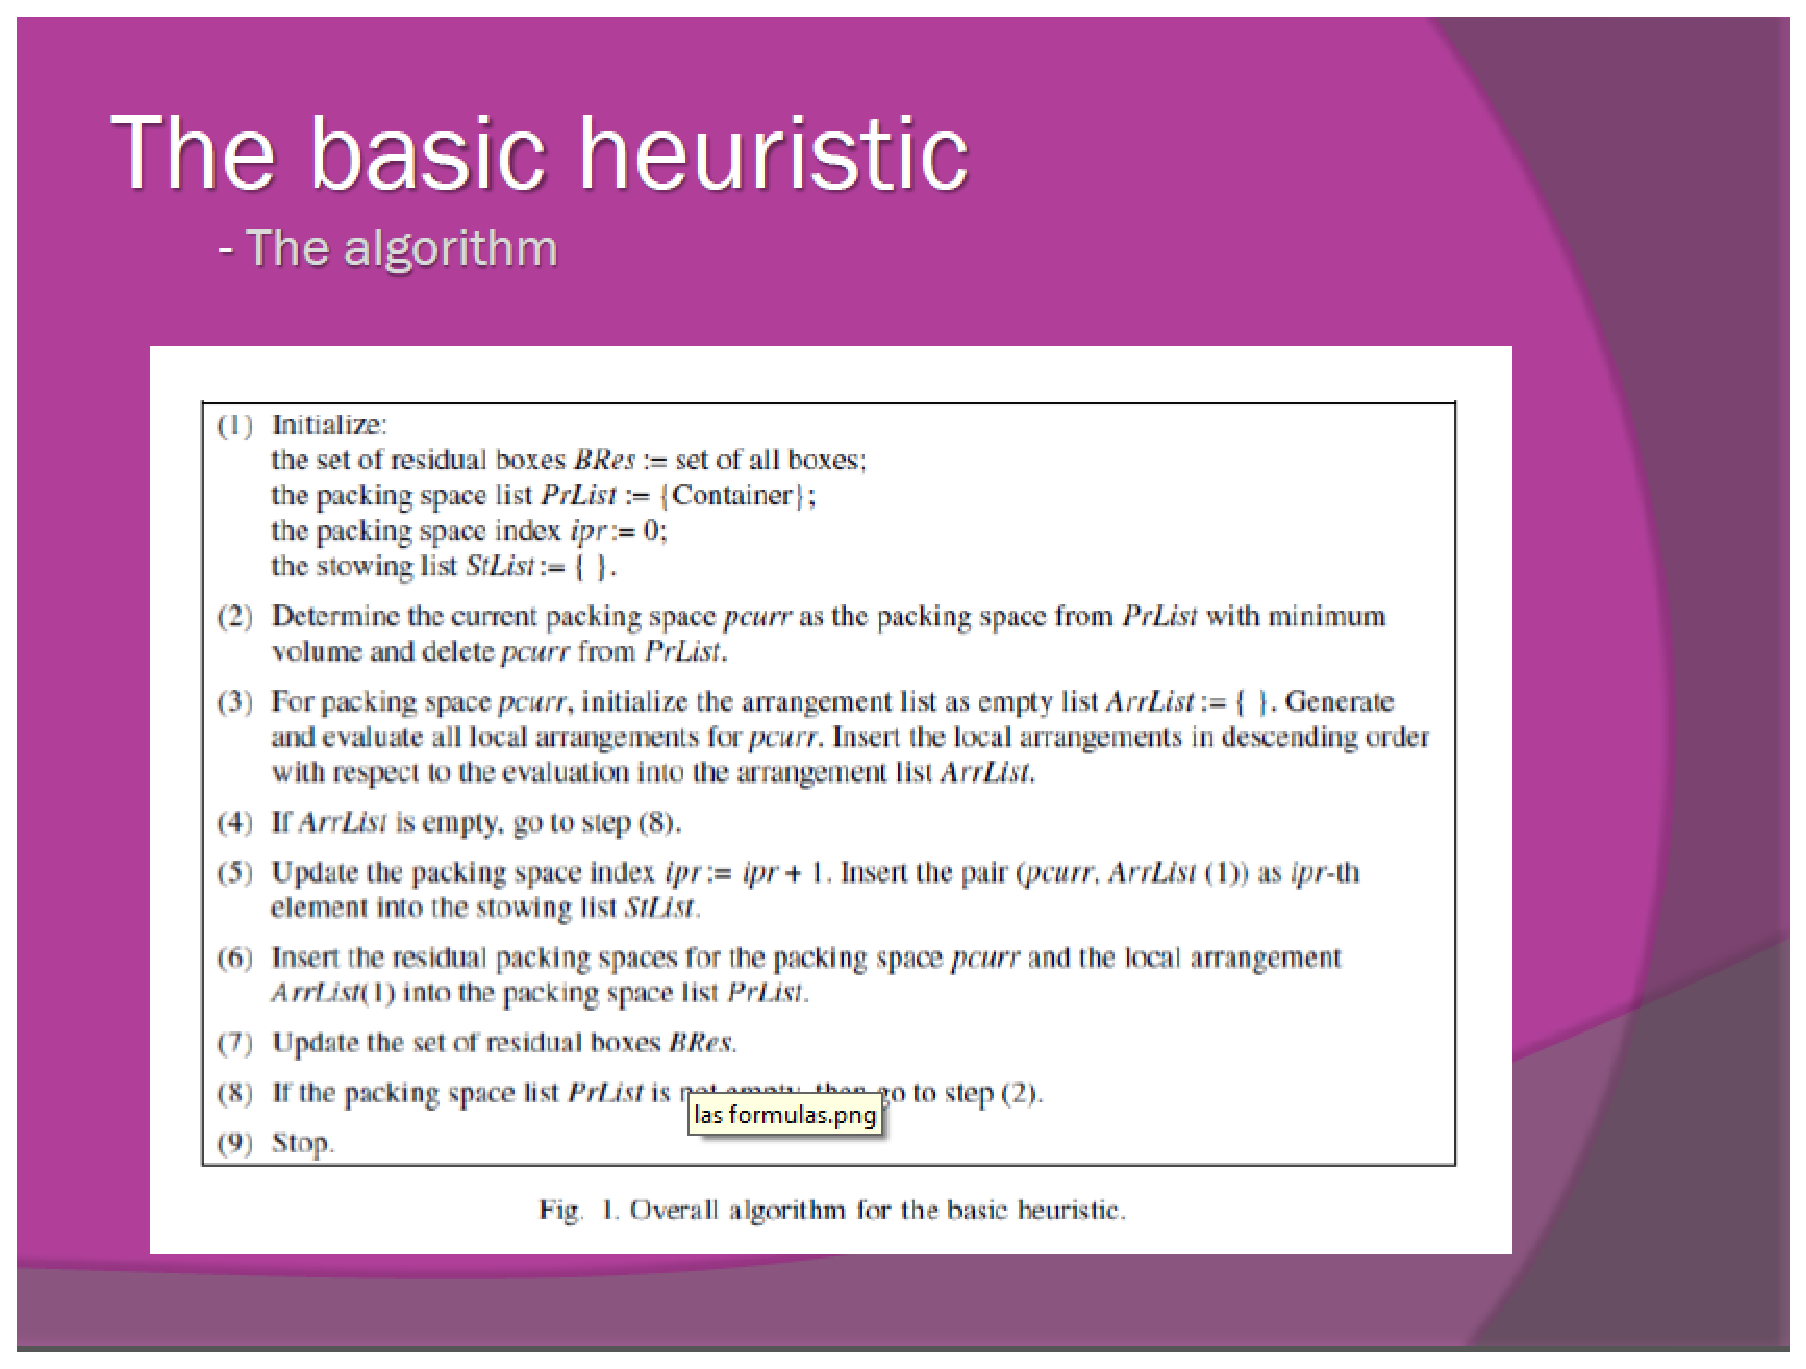
\includegraphics[width=1\textwidth]{images/picn5.eps}\\[0.25cm]
\end{center}

%%%%%%%%%%%%%%%%%%%%%%%%%%%%%%%%%%%%%%%%%%%%%%%%%%%%%%%%%%%%%%%%%%%%%%%%%%%%%%%
\chapter{Designing and alalizing }
\label{chapter:teo}

%%%%%%%%%%%%%%%%%%%%%%%%%%%%%%%%%%%%%%%%%%%%%%%%%%%%%%%%%%%%%%%%%%%%%%%%%%%%%%%
% Chapter 2: Fundamentos Teóricos 
%%%%%%%%%%%%%%%%%%%%%%%%%%%%%%%%%%%%%%%%%%%%%%%%%%%%%%%%%%%%%%%%%%%%%%%%%%%%%%%

%++++++++++++++++++++++++++++++++++++++++++++++++++++++++++++++++++++++++++++++

The structure of local arrangements for a packing space is defined as follows.
A local arrangement consists of one or two so-called blocks and is therefore referred
to as a 1- or 2-arrangement (see Fig. 2). A block is formed from boxes of
the same type. Furthermore, all boxes of a block are arranged in an identical spatial
orientation variant. In each of the three dimensions (x-, y- and z-direction) a block
consists of one or more boxes.
The only block of a 1-arrangement is always placed in the reference corner of the
packing space. From the two blocks of a 2-arrangement, one is arranged in the
reference corner. The second block can alternatively be placed as a neighbour in
x-direction (arrangement type ‘‘in front of’’), as a neighbour in y-direction (arrangement
type ‘‘beside’’) or as a neighbour in z-direction (arrangement type ‘‘above’’). In
the case of a placement according to arrangement type ‘‘in front of’’, the block with
the larger y-dimension is positioned in the reference corner, while for the arrangement
type ‘‘beside’’ the block with the larger x-dimension is positioned in the reference
corner. The arrangement type ‘‘above’’ is only used if both horizontal
dimensions of a block are not smaller than the corresponding dimensions of the
other block. The block with the larger horizontal dimensions is positioned in the reference
corner and the other above. Fig. 2 illustrates a 1-arrangement and two 2-
arrangements of the arrangement types ‘‘in front of’’ and ‘‘beside’’.
For the blocks of an arrangement, the box numbers in all three dimensions are
first determined in such a way that the concerned dimensions of the packing space
are utilized as fully as possible. If the number of boxes of a given type required
for a block exceeds the number of still available items of this type, then the numbers
of boxes are reduced appropriately.
With the selection of a box type and an orientation variant for its block, an 1-
arrangement is defined unambiguously. Analogously a 2-arrangement is completely
defined by the selection of two box types, two orientation variants, and an arrangement
type. All 1-arrangements and all 2-arrangements, which can occur if the box
types, the orientation variants and––in the case of 2-arrangements––the arrangement
type are varied, are generated. However, only those box types for which at least one
item is still available are considered here. Furthermore, the variation of the orientation
variants has to take the orientation constraint (C1) into consideration.

%++++++++++++++++++++++++++++++++++++++++++++++++++++++++++++++++++++++++++++++

%\section{Primer apartado del segundo capítulo}
%\label{2:sec:1}
%  Primer párrafo de la primera sección.

%\section{Segundo apartado del segundo capítulo}
%\label{2:sec:2}
%  Primer párrafo de la segunda sección.


%""""""""""""""""""""""""""""""""""""""""""""""""""""""""""""""""""""""""""""""
\begin{center}
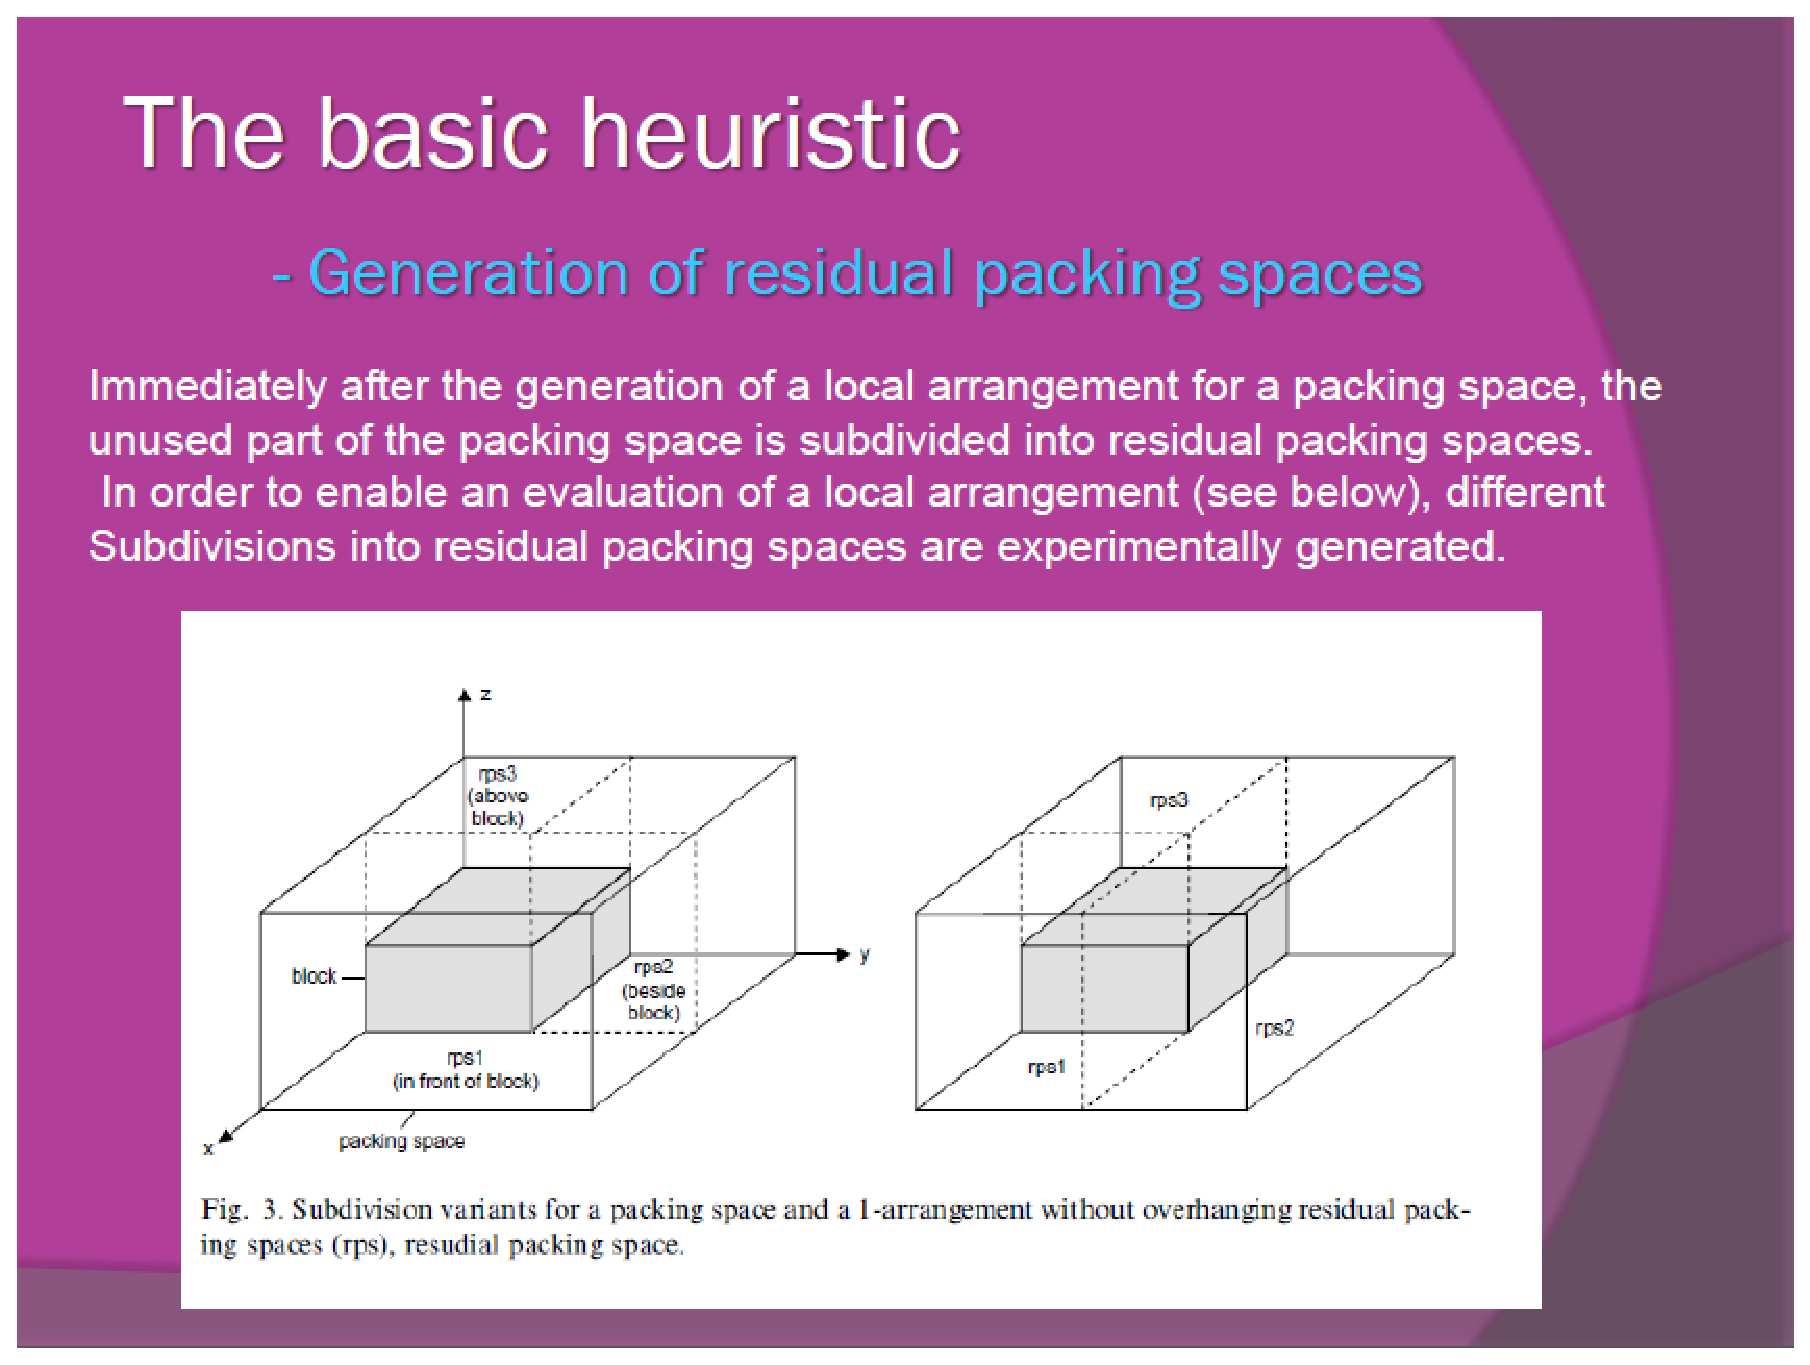
\includegraphics[width=1\textwidth]{images/picn7.eps}\\[0.25cm]
\end{center}
%""""""""""""""""""""""""""""""""""""""""""""""""""""""""""""""""""""""""""""""

%%%%%%%%%%%%%%%%%%%%%%%%%%%%%%%%%%%%%%%%%%%%%%%%%%%%%%%%%%%%%%%%%%%%%%%%%%%%%%%
\chapter{Technics of parallelization}
\label{chapter:exp}

%%%%%%%%%%%%%%%%%%%%%%%%%%%%%%%%%%%%%%%%%%%%%%%%%%%%%%%%%%%%%%%%%%%%%%%%%%%%%%%
% Chapter 3: Procedimiento experimental 
%%%%%%%%%%%%%%%%%%%%%%%%%%%%%%%%%%%%%%%%%%%%%%%%%%%%%%%%%%%%%%%%%%%%%%%%%%%%%%%


For the evaluation of the local arrangements generated for a packing space, two
modes are available which are applied alternatively. The selection of the relevant
mode is also controlled by a parameter, named arrEvalMode.
The first mode, encoded by the parameter value 0, applies a single evaluation criterion:
the total volume of the boxes stowed in the packing space which should be as
large as possible.
The second mode, encoded by the parameter value 1, additionally applies two further
evaluation criteria. These are the already introduced quantities loss volume and
maximum effective volume. Both criteria refer to the residual packing spaces of a local
arrangement. Analogous to the evaluation of subdivisions, the loss volume
should be as small as possible and the maximum effective volume as large as possible.
Since the three evaluation criteria applied are weighted equally, the evaluation procedure
is organized as a series of comparisons of the local arrangements for a packing
space in pairs.
Finally, two additional parameters of the basic heuristic are introduced and
briefly discussed. The parameter maxArr defines the maximum length of the arrangement
list ArrList for a packing space. A local arrangement is only considered in tabu search process if it occurs in ArrList, i.e. belongs to the maxArr best arrangements.
The parameter aboveArr determines whether 2-arrangements of type ‘‘above’’
are generated (parameter value 1) or not (parameter value 0). Like the different
modes for subdivisions and arrangements, the parameter aboveArr serves the diversi-
fication of the tabu searc

%++++++++++++++++++++++++++++++++++++++++++++++++++++++++++++++++++++++++++++++
%\section{Descripción de los experimentos}
%\label{3:sec:1}

%bla, bla, etc. 

%++++++++++++++++++++++++++++++++++++++++++++++++++++++++++++++++++++++++++++++
%\section{Descripción del material}
%\label{3:sec:2}

%bla, bla, etc. 


%++++++++++++++++++++++++++++++++++++++++++++++++++++++++++++++++++++++++++++++
%\section{Resultados obtenidos}
%\label{3:sec:3}

%bla, bla, etc. 


%------------------------------------------------------------------------------
%\begin{figure}[!th]
%\begin{center}
%\includegraphics[width=0.75\textwidth]{images/figura1.eps}
%\caption{Ejemplo de figura}
%\label{fig:1}
%\end{center}
%\end{figure}
%------------------------------------------------------------------------------


%------------------------------------------------------------------------------
%\input{tables/table.tex}
%------------------------------------------------------------------------------

%++++++++++++++++++++++++++++++++++++++++++++++++++++++++++++++++++++++++++++++
%\section{Análisis de los resultados}
%\label{3:sec:4}

%bla, bla, etc. 


%""""""""""""""""""""""""""""""""""""""""""""""""""""""""""""""""""""""""""""""
\begin{center}
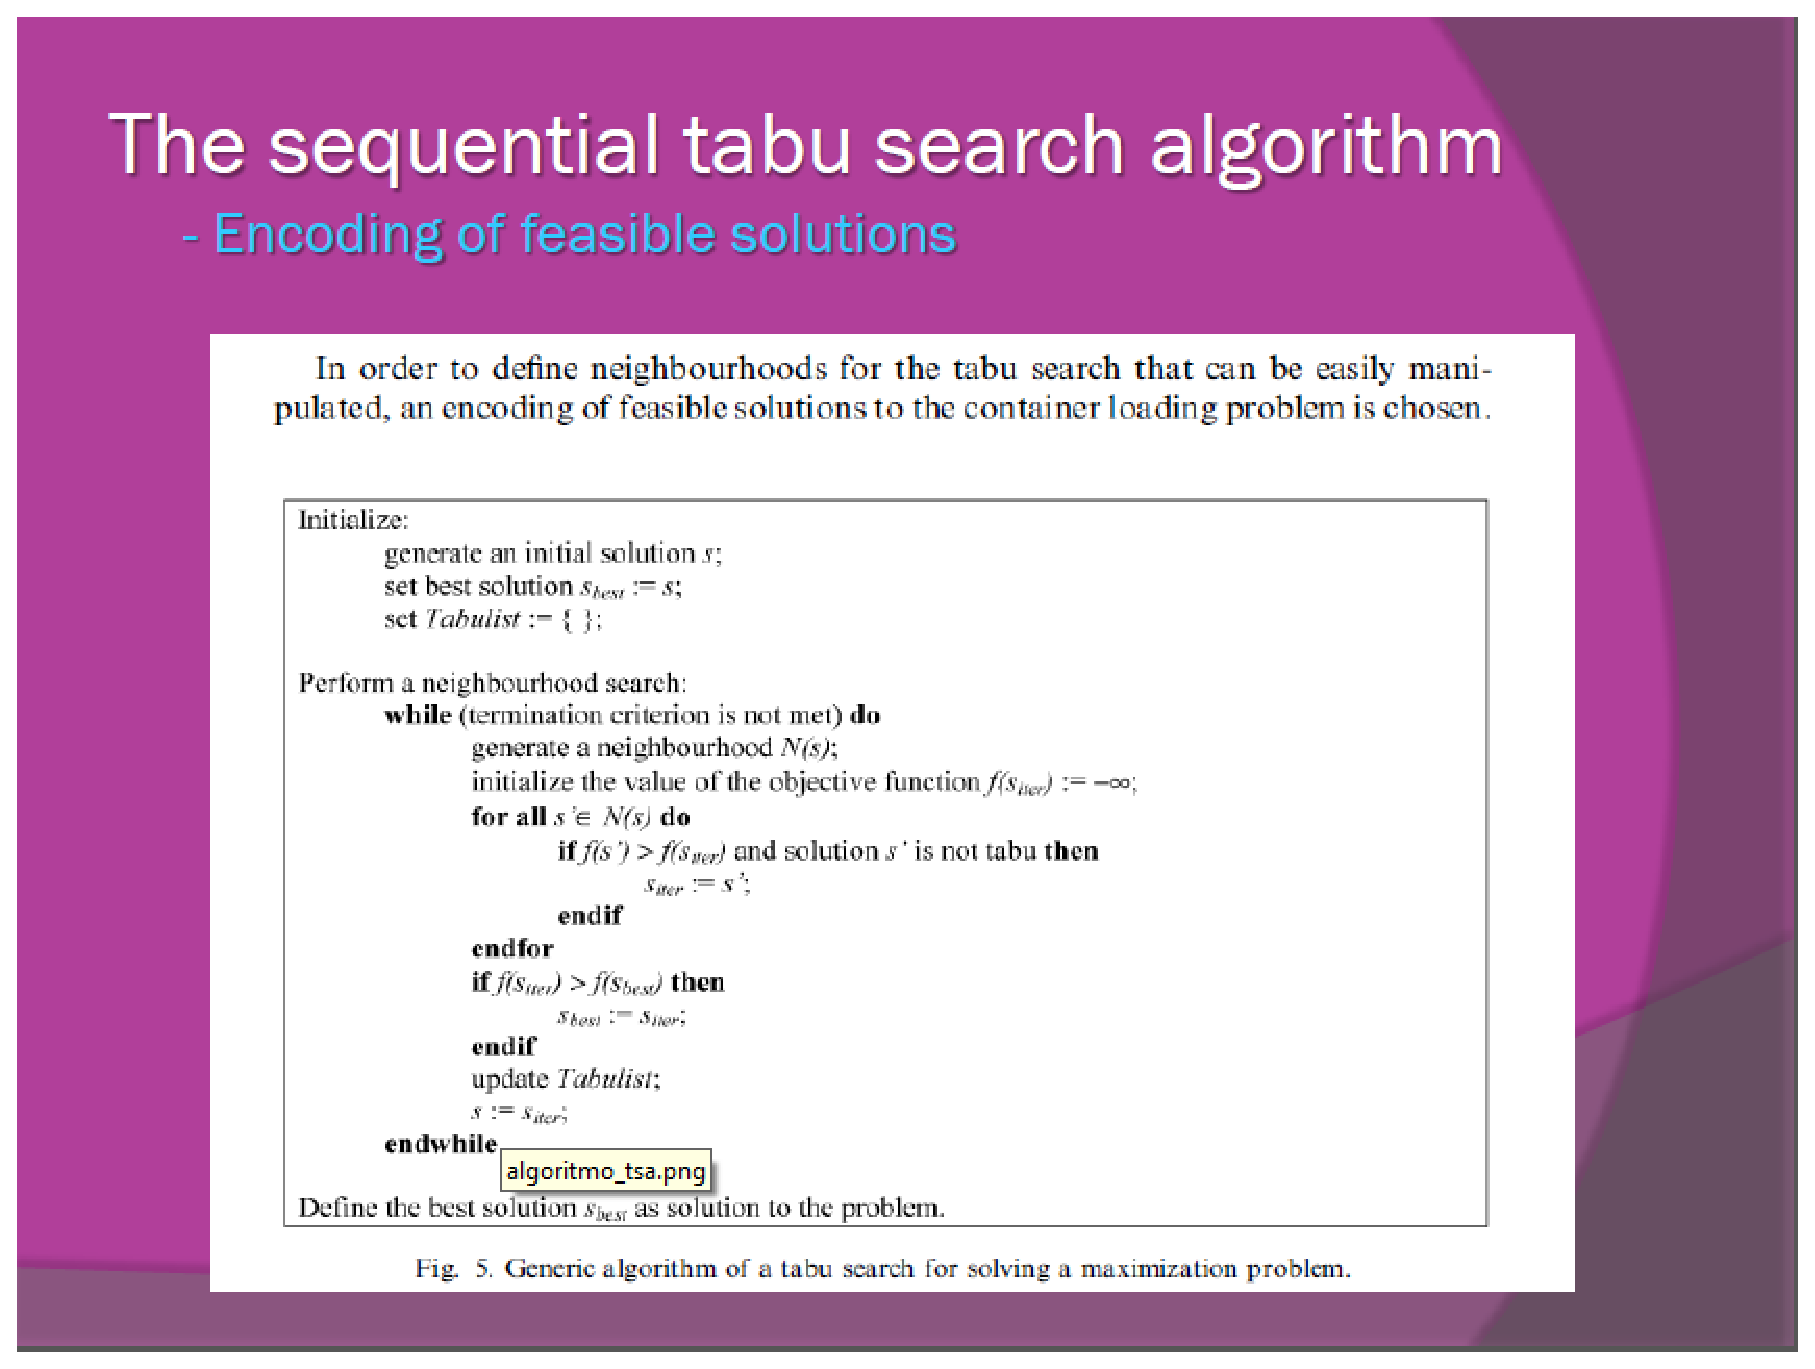
\includegraphics[width=1\textwidth]{images/picn11.eps}\\[0.25cm]
\end{center}
%""""""""""""""""""""""""""""""""""""""""""""""""""""""""""""""""""""""""""""""
%""""""""""""""""""""""""""""""""""""""""""""""""""""""""""""""""""""""""""""""
\begin{center}
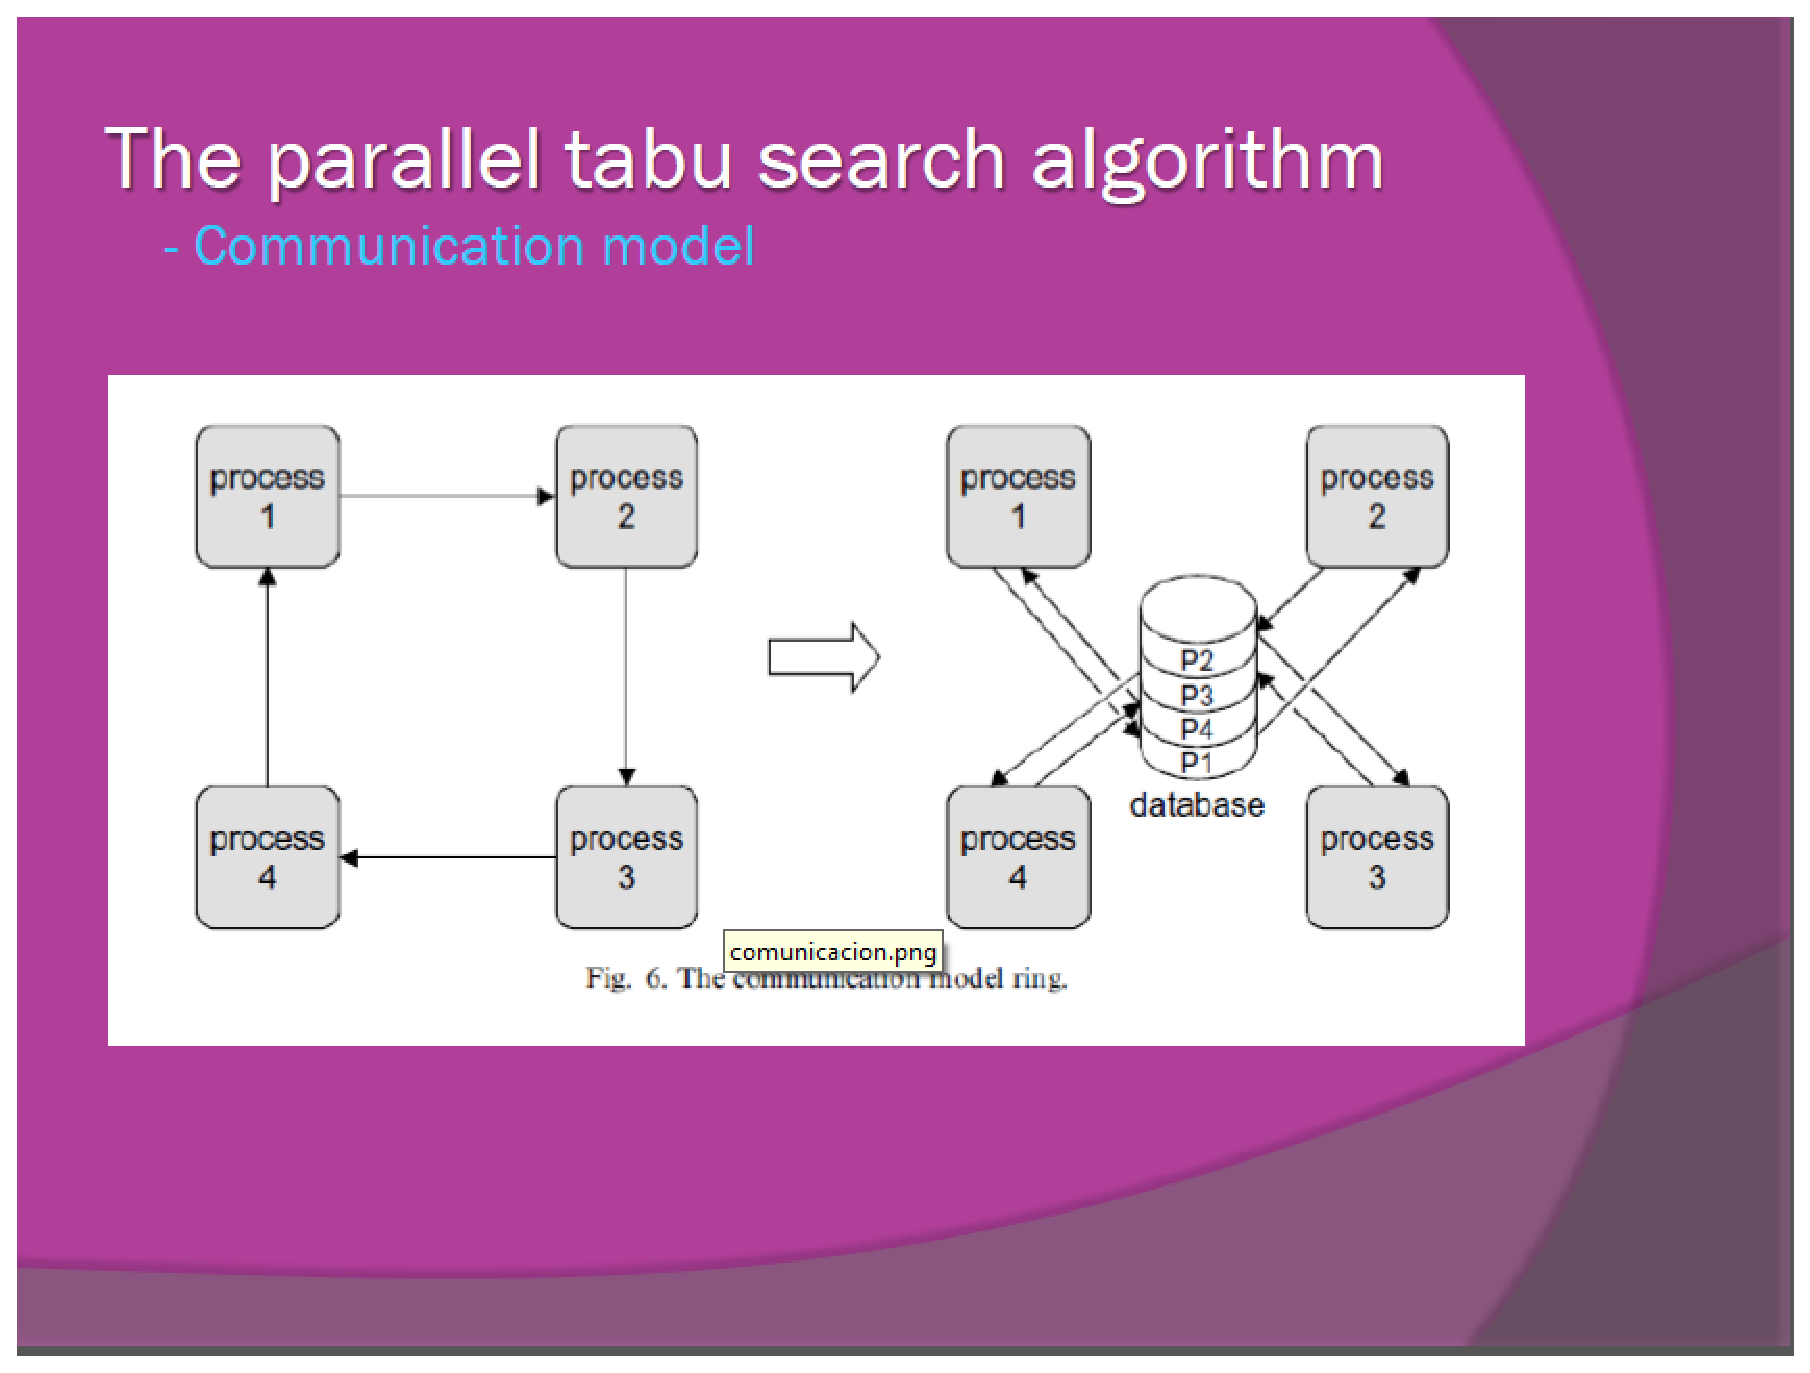
\includegraphics[width=1\textwidth]{images/picn12.eps}\\[0.25cm]
\end{center}
%%%%%%%%%%%%%%%%%%%%%%%%%%%%%%%%%%%%%%%%%%%%%%%%%%%%%%%%%%%%%%%%%%%%%%%%%%%%%%%
\begin{center}
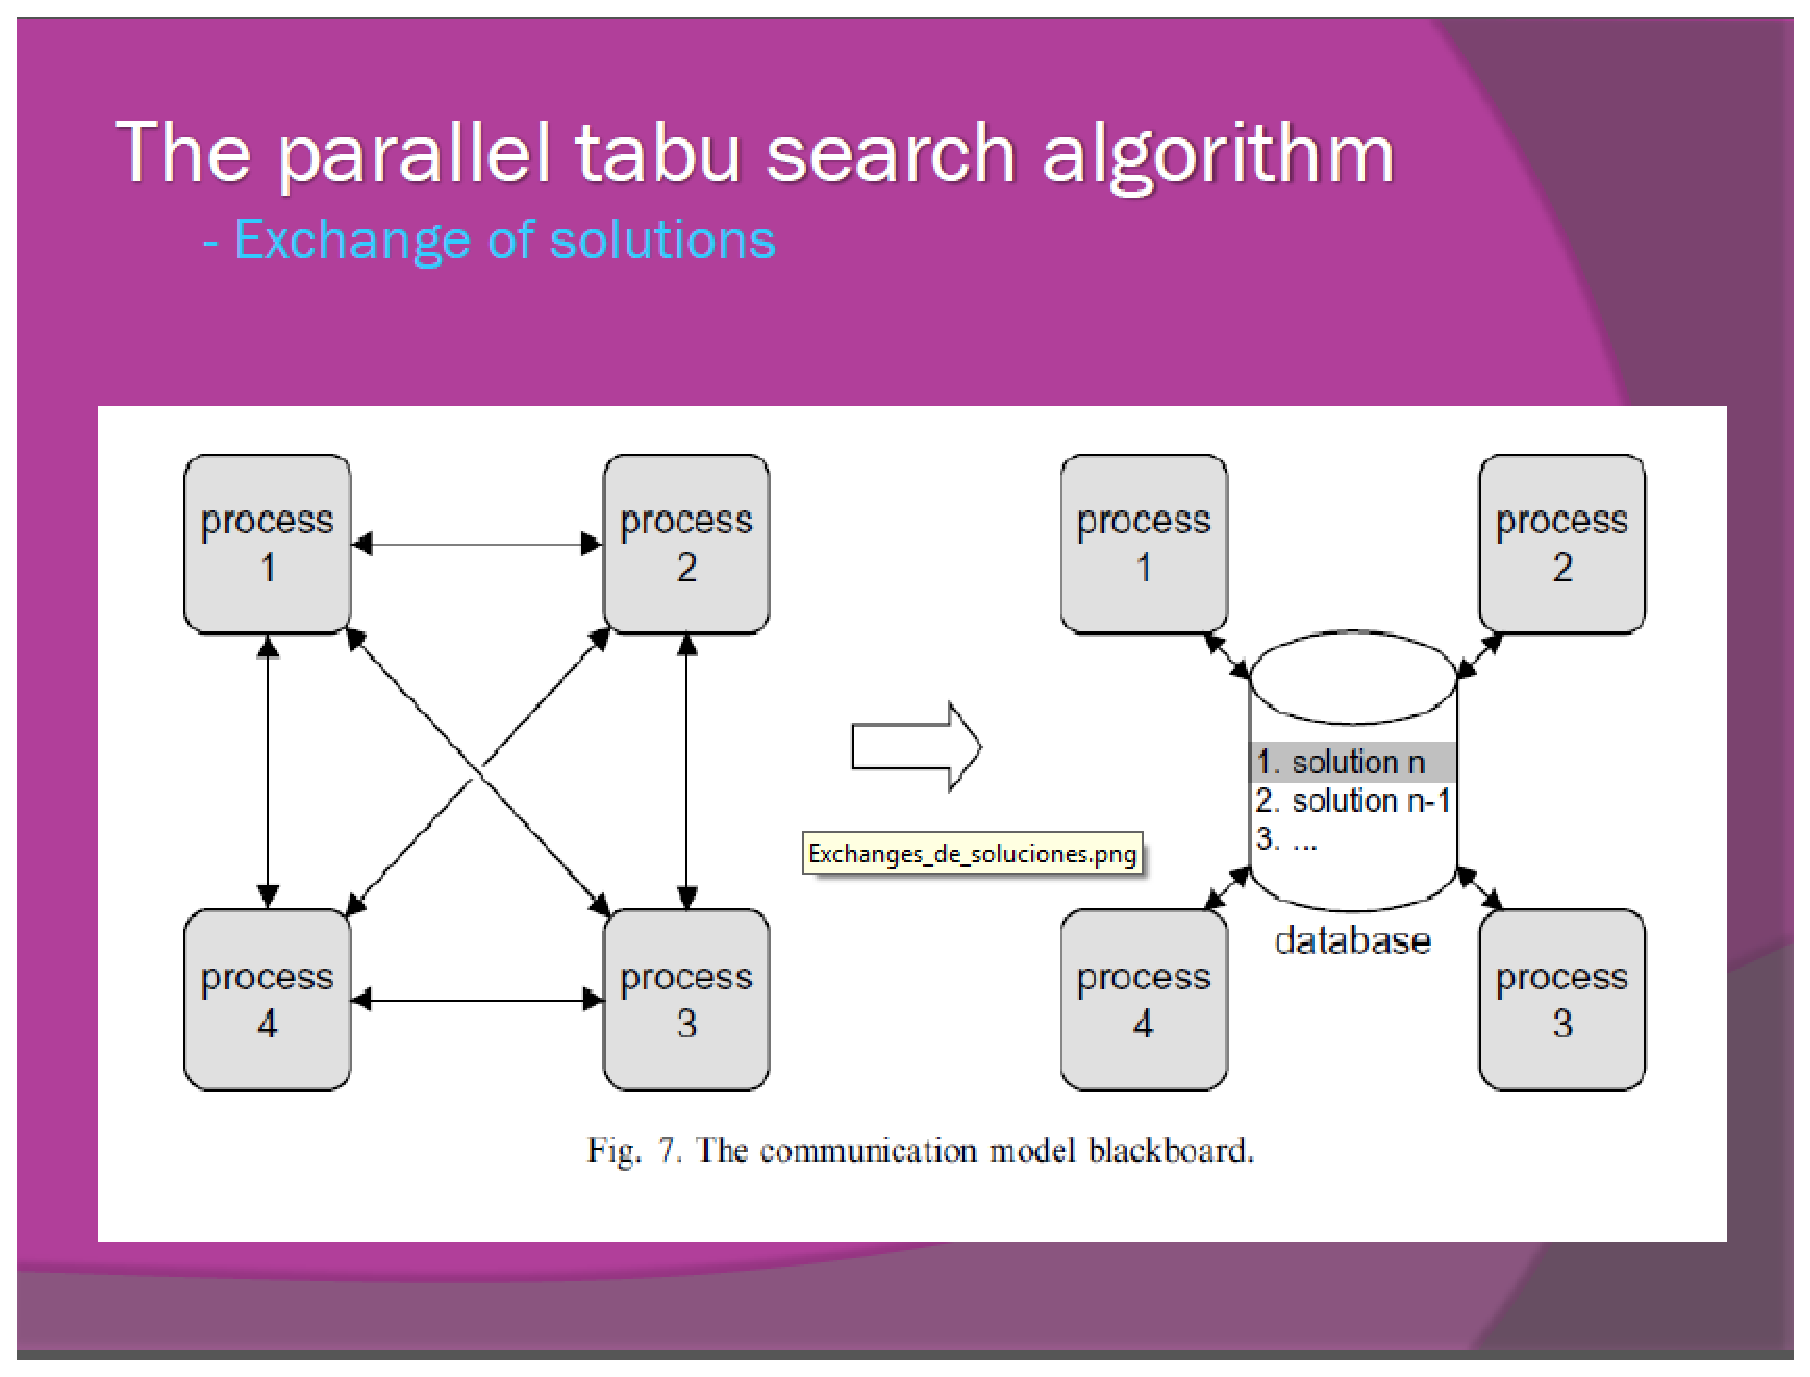
\includegraphics[width=1\textwidth]{images/picn14.eps}\\[0.25cm]
\end{center}
%%%%%%%%%%%%%%%%%%%%%%%%%%%%%%%%%%%%%%%%%%%%%%%%%%%%%%%%%%%%%%%%%%%%%%%%%%%%%%%
\begin{center}
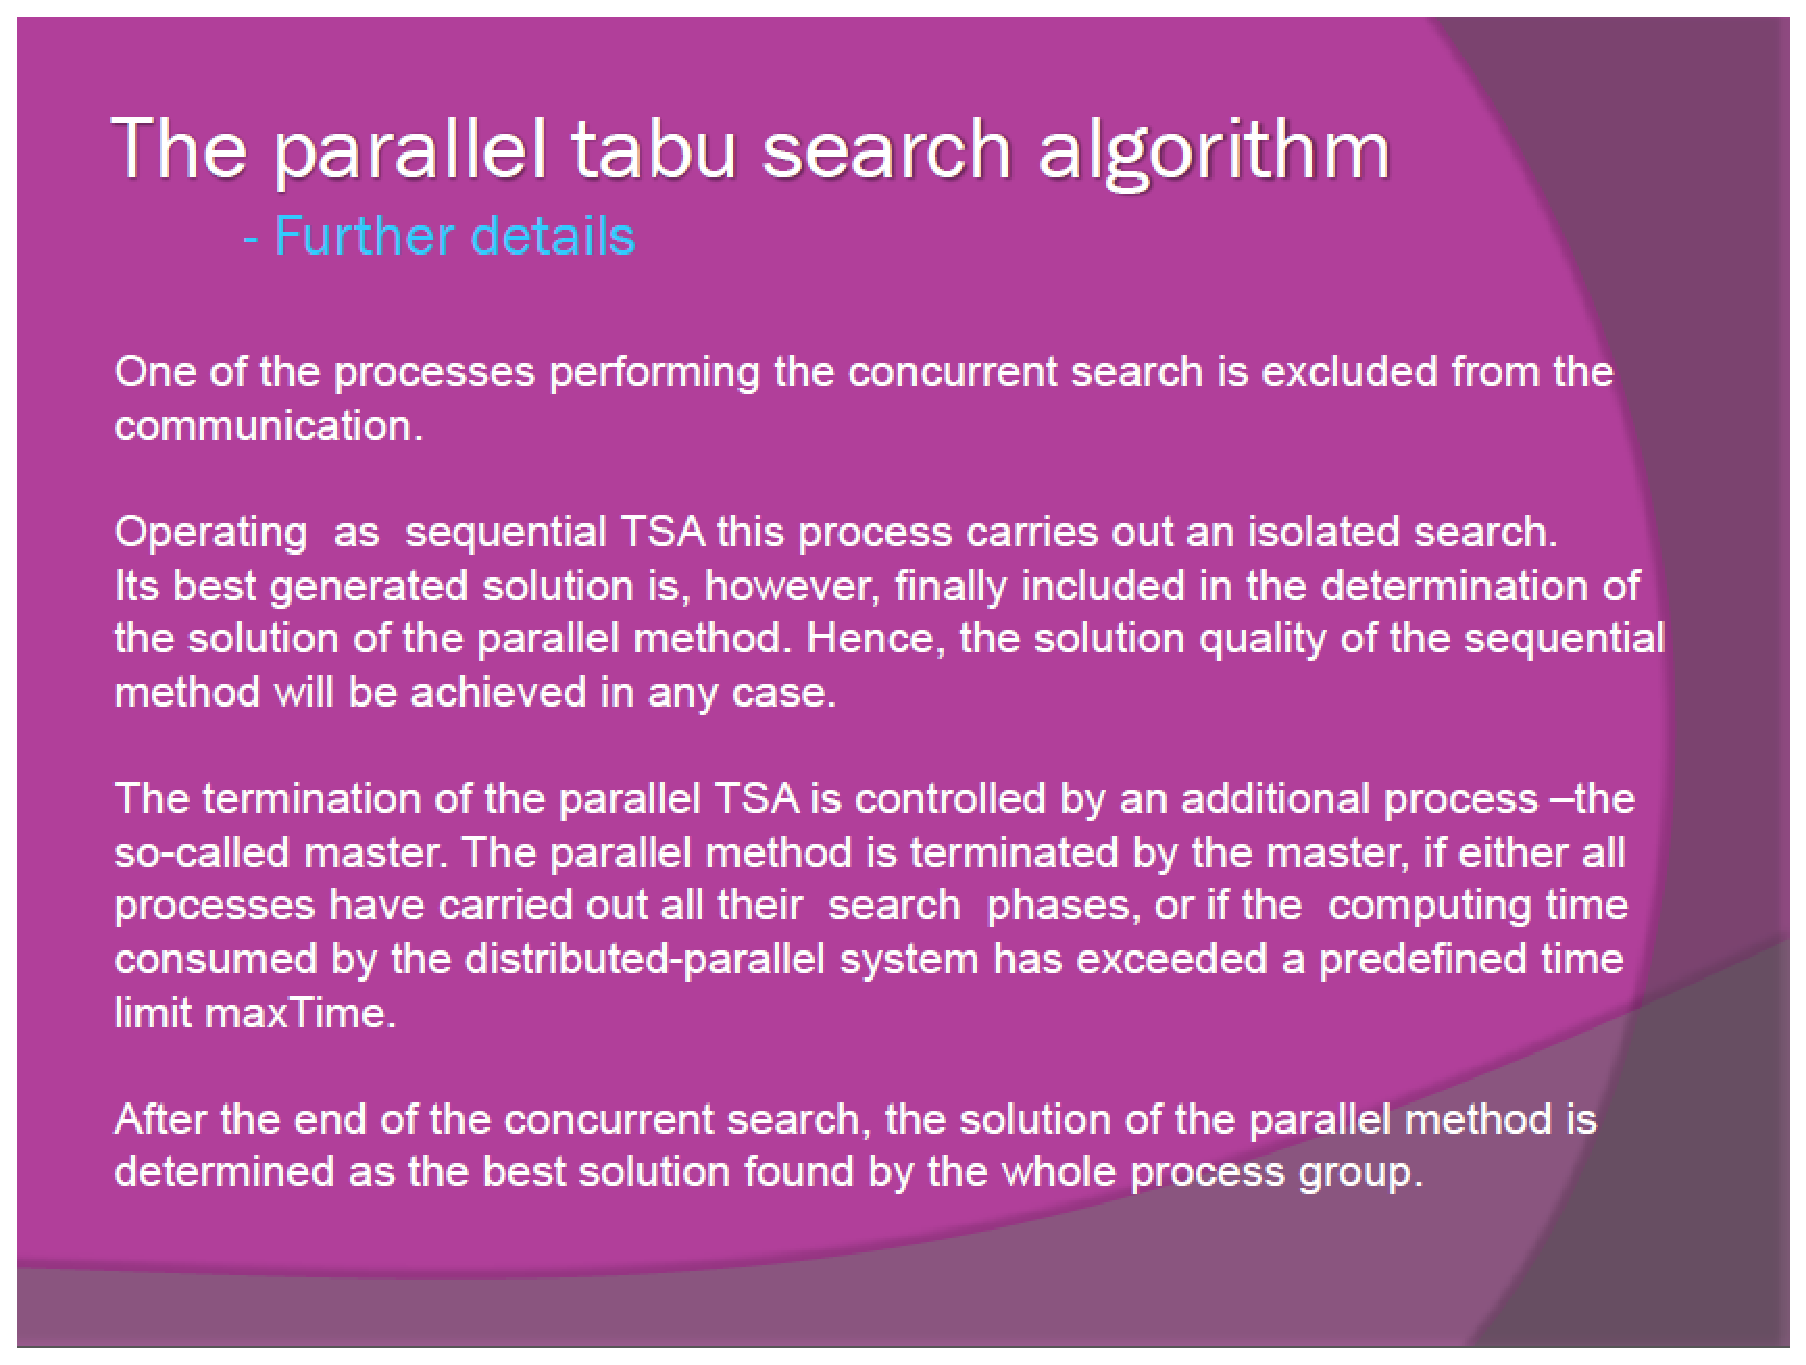
\includegraphics[width=1\textwidth]{images/picn15.eps}\\[0.25cm]
\end{center}
%""""""""""""""""""""""""""""""""""""""""""""""""""""""""""""""""""""""""""""""
%%%%%%%%%%%%%%%%%%%%%%%%%%%%%%%%%%%%%%%%%%%%%%%%%%%%%%%%%%%%%%%%%%%%%%%%%%%%%%%
\chapter{Conclusiones}
\label{chapter:conclusiones}

%%%%%%%%%%%%%%%%%%%%%%%%%%%%%%%%%%%%%%%%%%%%%%%%%%%%%%%%%%%%%%%%%%%%%%%%%%%%%
% Chapter 4: Conclusiones y Trabajos Futuros 
%%%%%%%%%%%%%%%%%%%%%%%%%%%%%%%%%%%%%%%%%%%%%%%%%%%%%%%%%%%%%%%%%%%%%%%%%%%%%%%


According to Toulouse et al. [20], three types of parallelization strategies seem to
be appropriate for the methods most often used in combinatorial optimization: (1)
parallelization of operations within an iteration of the solution method, (2) decomposition
of problem domain or search space, and (3) multi-search threads with various
degrees of synchronization and cooperation. Which of these types is suited for
the parallelization of an optimization method depends mainly on the goal pursued
by the parallelization. Since the enhancement of the solution quality is in the foreground
here, an approach of type 3 is chosen for the parallelization.
An instance of a container loading problem is treated by several processes. Each
process is an instance of the sequential TSA and solves the complete problem. However,
the individual instances are configurated differently. Furthermore, the processes
cooperate through the exchange of calculated solutions. A transmitted solution is
possibly used by the receiving process as a starting point for further search. While
the varying configuration of the processes causes a diversification of the search,
the exchange of solutions serves the intensification of the search within the regions
of best solutions.
Each of the autonomous processes is assigned to a workstation of a local network
(LAN). Hence, more precisely expressed, the parallel TSA is a distributed-parallel
method. It is described more closely in the following.
According to the diversification concept of the sequential TSA, the search in each
process is structured into several phases. In order to determine favourable parameter
settings with respect to the definition of the phases of all processes, a series of experiments
was carried out by means of the sequential TSA (cf. Section 5). The best parameter
settings are distributed approximately evenly over the processes and per
process the most promising parameter settings are, as far as possible, applied in early
phases. In this way the intended intensified exploration of regions that contain solutions
of high quality, is supported to a greater extent.
As to the communication frequency or the number of communications, the type
of the underlying sequential method (here a TSA) is to be considered. The consequence
of a very high communication frequency is that the individual processes
are prevented from intensively exploring limited regions of the search space. Therefore,
a lower communication frequency is to be chosen in advance. Here, an exchange
of best solutions is only carried out at the transition from one phase to the
next phase of each of the processes.
%""""""""""""""""""""""""""""""""""""""""""""""""""""""""""""""""""""""""""""""

%%%%%%%%%%%%%%%%%%%%%%%%%%%%%%%%%%%%%%%%%%%%%%%%%%%%%%%%%%%%%%%%%%%%%%%%%%%%%%%
\thispagestyle{empty}
%\begin{appendix}

%\chapter{Título del Apéndice 1}
%\label{appendix:1}

%\input{tex/apendice1.tex}

%\chapter{Título del Apéndice 2}
%\label{appendix:2}

%\input{tex/apendice2.tex}

%\end{appendix}

%%%%%%%%%%%%%%%%%%%%%%%%%%%%%%%%%%%%%%%%%%%%%%%%%%%%%%%%%%%%%%%%%%%%%%%%%%%%%%%
\addcontentsline{toc}{chapter}{Bibliografía}
\bibliographystyle{plain}


\bibliography{bib/references}

\nocite{*}

%%%%%%%%%%%%%%%%%%%%%%%%%%%%%%%%%%%%%%%%%%%%%%%%%%%%%%%%%%%%%%%%%%%%%%%%%%%%%%%

\end{document}
